
\documentclass[landscape,a0paper,fontscale=0.285]{baposter} 

\usepackage{graphicx} 
\graphicspath{{figures/}} 

\usepackage{amsmath} 
\usepackage{amssymb} 

\usepackage{booktabs} 
\usepackage{enumitem} 
\usepackage{palatino} 
\usepackage[font=small,labelfont=bf]{caption} 

\usepackage{multicol} 
\setlength{\columnsep}{1.5em} 
\setlength{\columnseprule}{0mm} 

\usepackage{tikz} 
\usetikzlibrary{shapes,arrows} 

\newcommand{\compresslist}{ 
\setlength{\itemsep}{1pt}
\setlength{\parskip}{0pt}
\setlength{\parsep}{0pt}
}

\definecolor{lightblue}{rgb}{0.145,0.6666,1} 

\begin{document}

\begin{poster}
{
headerborder=closed, 
colspacing=1em, 
bgColorOne=white, 
bgColorTwo=white, 
borderColor=lightblue, 
headerColorOne=lightblue, 
headerColorTwo=lightblue, 
headerFontColor=white, 
boxColorOne=white, 
textborder=roundedleft, 
eyecatcher=true, 
headerheight=0.1\textheight, 
headershape=roundedright, 
headerfont=\Large\bf\textsc, 
linewidth=2pt 
}

{
\includegraphics[height=5em]{gt1.png}} 
{\bf\textsc{Road Traffic Simulation}\vspace{0.5em}} 
{\textsc{\{ Stefan Henneking, Eisha Nathan, Lanssie Ma \} \hspace{12pt} Georgia Institute of Technology}} 
{
\includegraphics[height=4em]{gt2.png}} 

\headerbox{Problem Description}{name=problem,column=0,row=0}{

When modeling traffic flows along a busy, congested street, minimizing average travel time to traverse portions of streets becomes key. The objective of this project is to compare the average travel time for vehicles traveling along a portion of Peachtree Street in midtown Atlanta between a model using synchronized traffic lights versus unsynchronized traffic lights.

\vspace{0.3em} 
}


\headerbox{Input Analysis}{name=input,column=1,row=0,bottomaligned=problem}{


}

\headerbox{Results}{name=results,column=2,span=2,row=0, bottomaligned=input}{


}

\headerbox{Conceptual Model}{name=conceptual,column=0,below=problem}{ 
\begin{center}
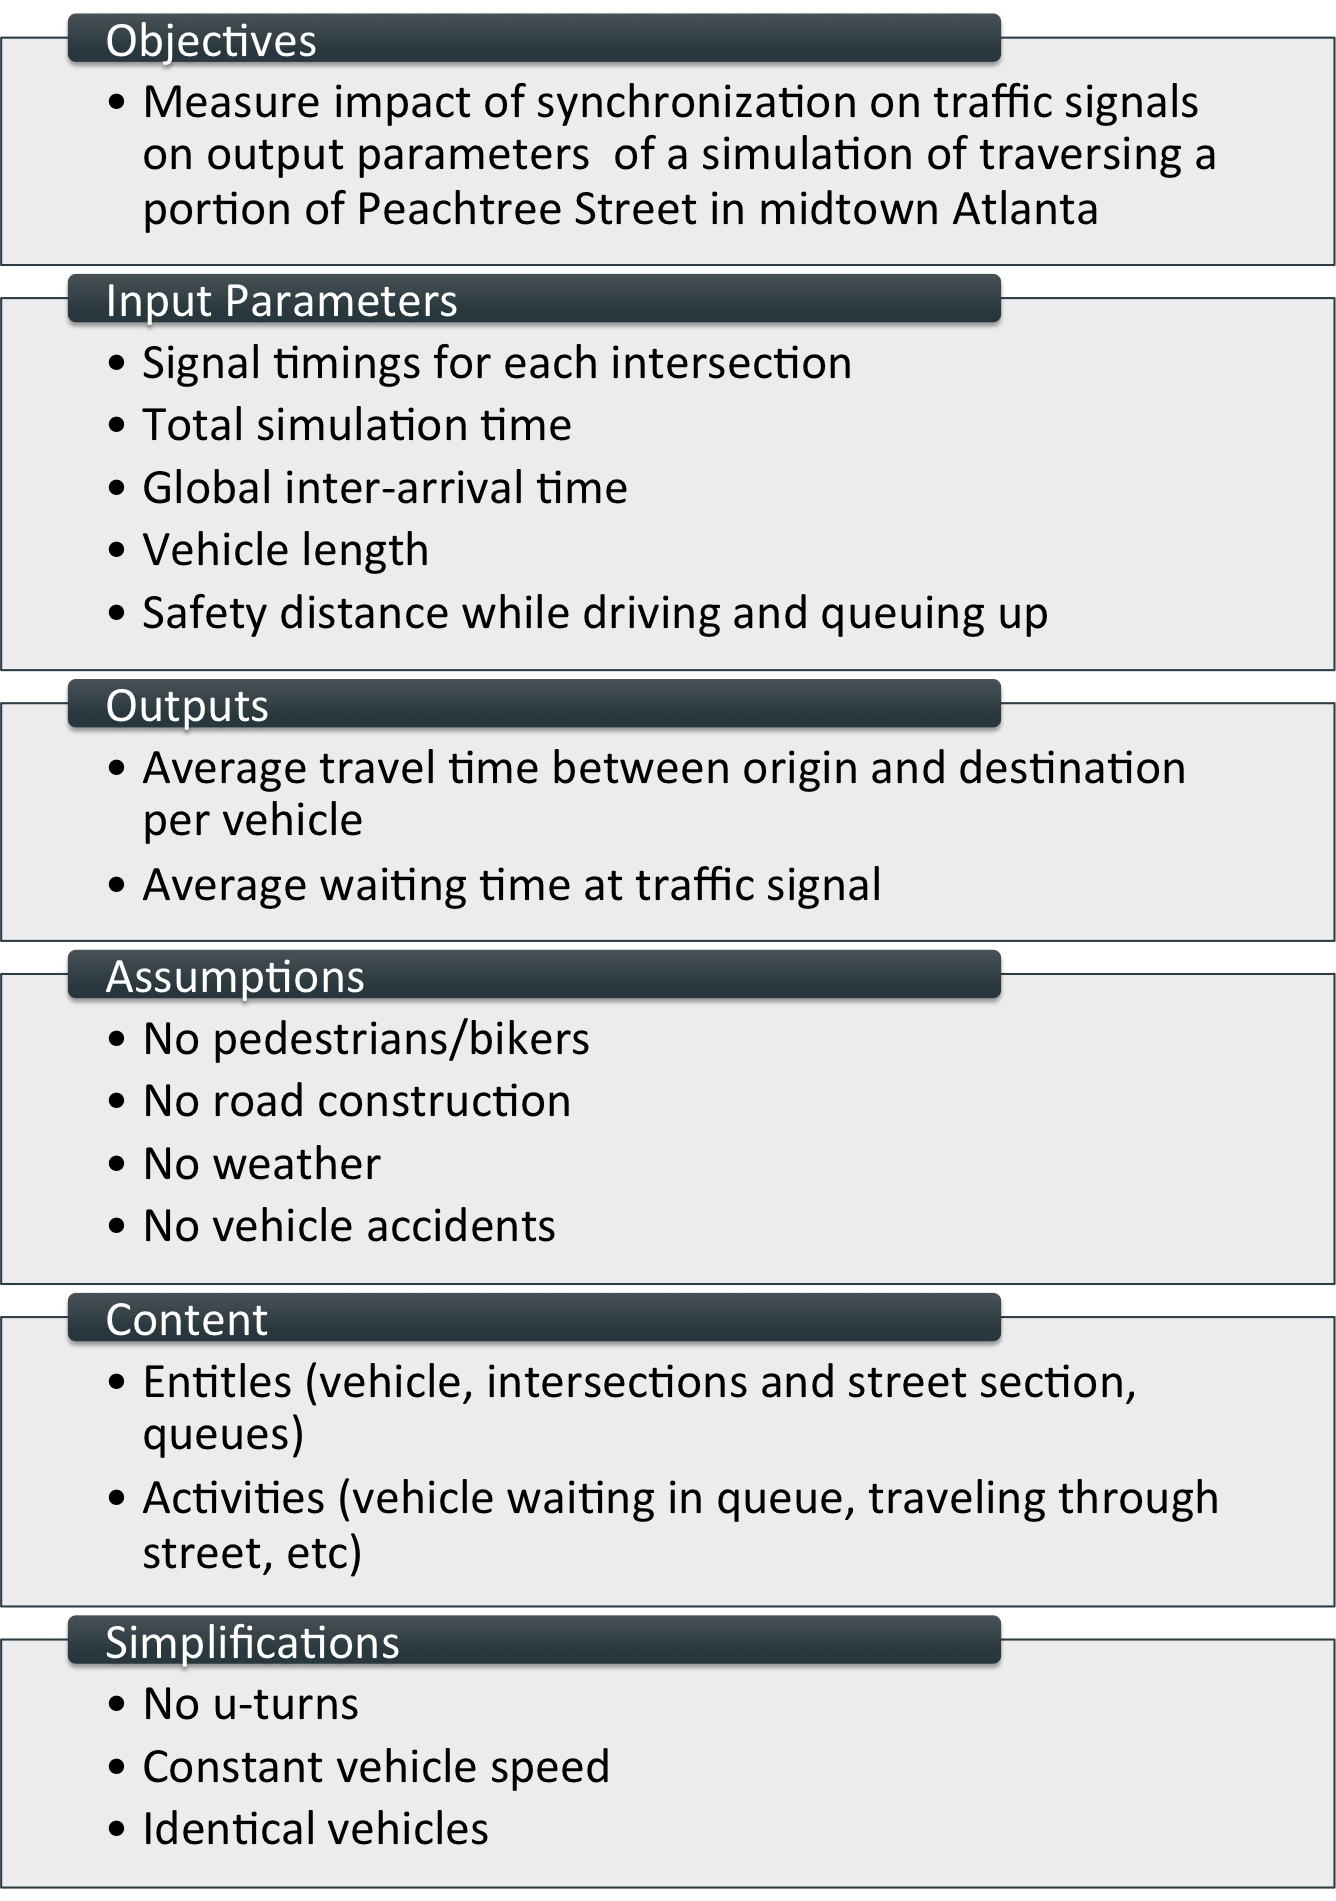
\includegraphics[width=1\linewidth]{cm}
\end{center}


}


\headerbox{Conclusion}{name=conclusion,column=2,span=2,row=0,below=results}{

Type conclusiony things here

}






\headerbox{Sample}{name=sample,column=0,below=conceptual,above=bottom}{ 


}

\headerbox{Implementation}{name=implementation,column=1,below=problem,bottomaligned=sample}{ 

\textit{Vehicle Queues \& Lanes}\\
Each lane is modeled as a queue and each queue is a linked list of events for vehicles; when the vehicle arrives at a particular intersection, it is placed in the appropriate lane queue. \\\\
\textit{Signal Lights \& Phases}\\

Each intersection structure contains an array containing the various stages of each light during each phase, and the current phase is kept track of as well as the total number of phases.
\begin{center}
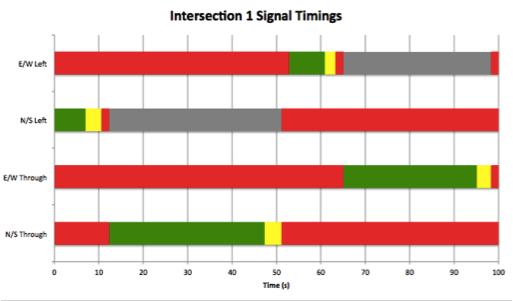
\includegraphics[width=.35\linewidth]{i1}

\end{center}

\textit{Intersection Event Handlers}\\
To simulate the switching of traffic lights, the current phase is incremented by 1. The next signal change will be scheduled using the current simulation time plus the time for the current phase as timestamp. First, after arriving at the intersection, the arrival event puts the vehicle is put into the corresponding lane queue. Next, the entering event prohibits any other vehicle from entering the intersection on this lane. The following crossing event is scheduled depending on on the vehicle acceleration, velocity, length and safety distance parameters. When the vehicle starts crossing the intersection, the next vehicle may enter and the departure event is scheduled. The intersection departure schedules either a new arrival at the following intersection or a global departure in case the vehicle is leaving the simulated roadway network.




}


\headerbox{Random Variables}{name=rv,column=2,span=2,bottomaligned=implementation,above=bottom}{ 

\begin{multicols}{2}
The C standard library rand() function is assumed to return uniformly distributed random values in the (0, R) interval such that rand()/R is uniform in (0,1), where R is an integral constant defined in the library. All input parameters were mapped to a uniform distribution except the inter-arrival time between vehicles, where an exponential distribution was used.

\begin{center}
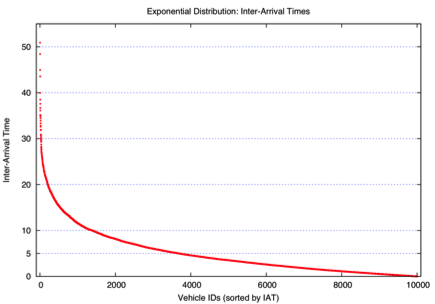
\includegraphics[width=.35\linewidth]{rv}
\captionof{figure}{Plot of IAT, $n$=10\,000, $\mu$= 5.}
\end{center}
\end{multicols}



}


\end{poster}

\end{document}